\documentclass{article}
\usepackage{titling}          % For å legge til undertittel
\usepackage{fontawesome5}      % For GitHub-symbolet
\usepackage{hyperref} 
\usepackage{graphicx} % Required for inserting images
\usepackage[utf8]{inputenc}
\usepackage[T1]{fontenc}
\usepackage{lmodern}
\usepackage[scaled]{beramono}
\usepackage[final]{microtype}
\usepackage{amssymb}
\usepackage{mathtools}
\usepackage{tikz}
\usepackage{algorithm}
\usepackage{lipsum}
\usepackage[noend]{algpseudocode}
\usepackage{amsmath}
\usepackage{bm}
\usepackage{tcolorbox}
\usepackage{hyperref}
\usepackage{multicol}
\setlength{\columnsep}{0.5cm} % Setter spalteavstand til 1 cm
\usepackage{amsthm}
\usepackage{thmtools}
\usepackage{babel}
\usepackage{caption}
\captionsetup[figure]{labelfont=bf, font=small}  % Setter "Figure X" i bold og tekst i liten skrift
\usepackage{titlesec} % For å tilpasse seksjon- og underseksjonsoverskrifter
\usepackage{textcase} % For å automatisk konvertere til caps

\usepackage{csquotes}
\usepackage{listings}
\lstset{basicstyle = \ttfamily}
\usepackage{textcomp}
\usepackage{siunitx}
\usepackage{xcolor}
\usepackage{tikz}
\usetikzlibrary{positioning}
\usepackage{graphicx}
\usepackage{float}
\usepackage{matlab-prettifier}
\usepackage[colorlinks, allcolors = uiolink]{hyperref}
\usepackage[a4paper, left=3.5cm, right=3.5cm, top=2.5cm, bottom=2.5cm]{geometry}

\newcommand{\EE}{\mathbb{E}}
\newcommand{\bb}[1]{\boldsymbol{#1}}
\newcommand{\ty}{\tilde{\bb{z}}}
\newcommand{\XX}{\mathbf{X}} 
\newcommand{\VV}{\mathbf{V}} 
\newcommand{\UU}{\mathbf{U}} 

% Format for seksjonsoverskrifter
\titleformat{\section}
  {\centering\bfseries\MakeTextUppercase} % Midtstilt, bold, caps
  {\thesection}{1em}{} % Nummereringsformatet for seksjon

% Format for underseksjonsoverskrifter (venstrestilt, bold, samme størrelse som brødtekst)
\titleformat{\subsection}
  {\bfseries} % Bold, samme størrelse som brødtekst (12pt)
  {\thesubsection}{1em}{} % Nummereringsformatet for subseksjon

% Format for underseksjonsoverskrifter (venstrestilt, bold, samme størrelse som brødtekst)
\titleformat{\subsubsection}
  {\bfseries} % Bold, samme størrelse som brødtekst (12pt)
  {\thesubsection}{1em}{} % Nummereringsformatet for subseksjon

\setlength{\parskip}{0pt} % Fjerner mellomrom mellom avsnitt
\setlength{\parindent}{15pt} % Beholder innrykk

% Fjerne ekstra mellomrom mellom underseksjon og tekst
\titlespacing{\subsection}{0pt}{*1}{*0} % Ingen vertikal plass før eller etter subsection
\titlespacing{\subsubsection}{0pt}{*1}{*0} % Ingen vertikal plass før eller etter subsection

%%%%%%%%%%%%%%%%%%%%%%%%%%%%%%%%%%%%%%%%%%%%%%%%%%%%%%%%
%                   TITTEL/CREDITS                     %
%%%%%%%%%%%%%%%%%%%%%%%%%%%%%%%%%%%%%%%%%%%%%%%%%%%%%%%%

% Håkon la inn denne tittelen bare for å være i gang, selv om det ikke er sikkert at det er sånn vi vil gjøre det
\title{Sleep Scoring in Alzheimer Mouse Models: Comparing Traditional and Spatial Approaches using Feed Forward and Convolutional Neural Networks}

\author{Oscar Atle Brovold, Eskil Grinaker Hansen, Håkon Ganes Kornstad}
\date{December 8, 2024}

\begin{document}
\maketitle
\begin{center}
    \href{https://github.com/EOH-ML/FYS-STK3155-Projects/tree/main/project3}{\texttt{Project GitHub Repository}}
\end{center}

%%%%%%%%%%%%%%%%%%%%%%%%%%%%%%%%%%%%%%%%%%%%%%%%%%%%%%%%
%                   ABSTRACT/INTRO                     %
%%%%%%%%%%%%%%%%%%%%%%%%%%%%%%%%%%%%%%%%%%%%%%%%%%%%%%%%

\begin{abstract}
\noindent 
It is established that sleep plays a role in Alzheimer’s Disease, influencing processes that may impact disease progression. Sleep scoring, vital for understanding these mechanisms, is typically labor-intensive and performed manually. Automating sleep scoring with machine learning is therefore potentially a great tool for improving the efficiency in Alzheimer research. We build two machine learning models for sleep scoring in mice based on the same dataset of 14 different test mouse models. Datasets are from trials measuring brainwaves with Electrocorticography (ECoG) and muscle activities with Electromyography (EMG). We train our Feed Forward Neural Network (FFNN) in tandem with an extensive feature engineering, yielding an overall accuracy of 87\%, as well as F1-scores of 67\% and 48\% on Intermediate Sleep (IS) and REM, respectively. Then we compare it to a CNN-model with two convolution layers, kernel size \texttt{(2, 2)} and \texttt{MaxPooling}, using ReLU as activation function in the dense layers. It is trained on plots of ECoG and EMG in the frequency domain, and yields an overall accuracy of 92\%, and sleep stage individual F1-scores of 74\% and 69\% on IS and REM, respectively. We conclude that while FFNNs can effectively learn diverse tasks, the CNN outperforms it in our testing. We propose this is due to the CNN's ability to extract spatial patterns from frequency-domain data, making it better suited for sleep scoring.

% We conclude that a further extension of the CNN-model using a Hidden Markov Model (HMM), as well as more high definition data could further improve the results.
\end{abstract}

\section*{INTRODUCTION}
\begin{multicols}{2}
Sleep Scoring is used to determine the vigilance state of an organism, typically distinguishing between states like \textit{wakefulness}, \textit{REM} (Rapid Eye Movement), and \textit{non-REM} sleep. Traditionally, sleep scoring in mammals is performed manually by an expert, by comparing the dominance of certain brain waves across different frequency bands. This is a repetitive and labour intensive work. An automated sleep scoring algorithm would therefore save time and free up the researchers to do other work.

\textit{GliaLab} is a Norwegian research group at the Medical Department of The University of Oslo (UiO). It conducts research on the role of glial cells, particularily \textbf{astrocytes}. It is thought that these cells are important in slowing down the progression of Alzheimer’s Disease (AD) and Parkinson’s Disease, by clearing particles that contribute to amyloid placque formation in the Hippocampus. \cite{enger_glialab_nodate} Astrocytes operate mainly in the area around the blood vessels, the \textbf{perivascular space} \cite{bojarskaite_sleep_2023}. Observing the brain of test mice with AD during sleep, \textit{GliaLab} investigates how the vascular contraction in each vigilance state contribute to opening up the perivascular space, thus facilitating the astrocytes in their cleaning work. \cite{bojarskaite_sleep_2023}

There have been several experiments on using increasingly advanced machine learning models for sleep scoring in recent years. \cite{alattar_artificial_2024} \cite{aboalayon_sleep_2016} This can be credited to the advancements in hardware, and the access to increasingly extensive health data. \cite{alattar_artificial_2024} Being three bachelor students in the subject FYS-STK3155 \textit{Applied Machine Learning} at the University of Oslo, we are grateful to be granted access to the data from \textit{GliaLab}'s mouse trials. 

We aim to implement and then compare a standard Feed Forward Neural Network (FFNN), with a slightly simplified version of one of the most successful Convolutional Neural Network (CNN) models, namely \textit{SPINDLE} \cite{miladinovic_SPINDLE_2019}, trained on frequency plots. For both networks we also make use of feature enginering to further enhance the data according to domain knowledge. We focus on using precision, accuracy and F1-score as our main metrics, both globally and per sleep stage, for comparing the FFNN and CNN models' performance. \end{multicols}

%%%%%%%%%%%%%%%%%%%%%%%%%%%%%%%%%%%%%%%%%%%%%%%%%%%%%%%%
%                       TEORI                          %
%%%%%%%%%%%%%%%%%%%%%%%%%%%%%%%%%%%%%%%%%%%%%%%%%%%%%%%%
\section*{Theoretical background}

\begin{multicols}{2}
\subsection*{Trials in Mouse Models at \textit{GliaLab}}
An opening in the mouse models’ skull revealing the brain’s blood vessels is observed under a two-photon microscope. This enables the researchers to find correlations of sleep patterns with vascular contractions, and the accumulation of the AD-related amyloid placque. If sleep plays a role in the drainage of the agents that accumulate amyloid placque, it would be of great value to assess the sleep stages of the mouse in trial. \cite{bojarskaite_sleep_2023}

\begin{figure}[H]
    \centering
    \includegraphics[width=\columnwidth]{figures/mouse_scope2.eps} 
    \caption{A two-photon microscope photographs the brain of a mouse, showing the vascular contractions during different sleep stages. By attaching Electrocorticography (EcOG)-electrodes on the model, brainwave activity can be measured in real time. In parallel, electromyography (EMG) electrodes are mounted on the model’s neck musculature, tracking the mouse model’s movement. Both the EcOG and EMG data is used in manual sleep scoring. \textbf{Illustration of mouse:} \textit{BioRender}, used with an Open Source permission.}
    \label{fig:mouse_fig}
\end{figure}

\section*{Sleep Scoring}
\subsubsection*{Electrocorticography (ECoG)}
ECoG is a method for measuring electrical activity in the brain. Unlike EEG, where electrodes are placed \textit{on} the scalp, ECoG electrodes are placed directly on the surface of the cerebral cortex through surgery. This provides ECoG with better spatial resolution and stronger signal strength compared to EEG, making it less susceptible to artifacts such as noise. \cite{halnes_electric_2024}

\subsubsection*{Electromyography (EMG)}
The electromyogram (EMG) measures electrical activity in muscles, and thereby tracking movement across different sleep stages. An electrode is mounted on the neck musculature to infer changes in motor activity associated with wakefulness, non-rapid eye movement (NREM), and rapid eye movement (REM) sleep. During wakefulness, EMG signals typically exhibit high-amplitude, irregular bursts due to active movement. In contrast, NREM sleep is characterized by a reduction in muscle tone, with lower-amplitude, more stable EMG signals. REM sleep is marked by a near-complete loss of muscle tone, resulting in minimal or absent EMG activity. \cite{engstrom_elektromyografi_2024}

\subsection*{Machine Learning based Sleep Scoring Setups}
Machine learning for sleep scoring has been explored for decades. However, it remains challenging to develop models that perform well across the diverse genetic backgrounds of mouse models and their varied research environments. Similarly, these models often fail to generalize to other mammals, making them unsuitable for human sleep scoring. Despite these challenges, the significant amount of time spent annually by research groups on manual sleep scoring makes it worthwhile to continue pursuing automated approaches. \cite{alizadeh_savareh_performance_2018}

Our CNN model is inspired by \textit{SPINDLE}, a model developed at ETH Zurich in 2019, and collaborating institutions. \textit{SPINDLE} employs a CNN architecture, complemented by a hidden Markov model (HMM), to generalize sleep stage predictions across experimental settings, species, and labs. The study obtains an impressive overall accuracy of 93-99\%. For the hard-to-predict REM-stage, they offer a F1-score ranging between 85-98\%, dependent on animal cohorts and the addition of HMM. \cite{miladinovic_SPINDLE_2019}

\subsubsection*{Feed Forward Neural Network (FFNN)} 
A Feed Forward Neural Network (FFNN) is a basic artificial neural network. Information flows sequentially from the input layer, through a series of hidden layers, and finally to the output layer. FFNNs are highly versatile and often deliver strong results across a wide variety of machine learning tasks. For the underlying theory and training methodology of FFNNs, please refer to the section on Feed Forward Neural Networks in our Report 2 \cite{brovold_less_2024}.


\subsubsection*{Convolutional Neural Networks}
Convolutional Neural Networks (CNNs) are a specialized class of neural networks, well-suited for analyzing visual data. Unlike standard feed-forward neural networks \cite{brovold_less_2024}, CNNs incorporate convolution layers that are useful for recognizing patterns, such as edges and textures. Following the convolutional layers, the CNN further applies fully connected layers, similar to traditional feed-forward networks. This specialized structure aims to effectively solve tasks such as image recognition, object detection, and other applications involving spatial data. \cite{goodfellow_deep_2016}

Each convolutional layer consists of three stages; a \texttt{convolution stage}, a \texttt{detection stage} and finally a \texttt{pooling stage}.

\begin{figure}[H]
    \centering
    \includegraphics[width=\linewidth]{figures/convolution_goodfellow.eps} 
    \caption{The convolution stage, convolving a $3\times 4$ image with a $2\times 2$ kernel. (Freely after Illustration 9.1 in Goodfellow et al.\cite{goodfellow_deep_2016})}
    \label{fig:convolution}
\end{figure}

The convolution stage is illustrated in \hyperref[fig:convolution]{Figure~\ref*{fig:convolution}}, and is for most machine learning purposes mathematically defined as:
$$S(i, j) = \sum_m \sum_n I(i-m, j-n) K(m, n)$$
Here $I$ is the two-dimensional image and $K$ is the kernel/filter (a weighted matrix). $S(i, j)$ is the output, which is sometimes referred to as the \textbf{feature map} \cite{goodfellow_deep_2016}. This process is useful for extracting specific features of $I$. The next stage of the convolutional layer is a \textbf{detection stage} — here we apply a non-linearity, e.g the rectified linear unit (ReLU). The final step is the so-called \textbf{pooling stage}, implemented to downsample the feature map. This is done by calculating a ``summary statistic'' for a certain location based on nearby outputs. This speeds up calculation and possibly reduces overfitting. Some common pooling strategies consists of \textbf{max pooling}, \textbf{average pooling} and \textbf{$L^2$ pooling}. Finally, the output of the last convolutional layer is flattened and sent through a series of \textbf{fully connected} (``dense'') layers, yielding the final prediction.
\cite{goodfellow_deep_2016}

\subsubsection*{Evaluation Methods}
When dealing with classification tasks there are several methods to evaluate a model's predictions on a test set of data. 

\begin{figure}[H]
    \centering
    \includegraphics[width=\linewidth]{figures/conf_matrix.eps} 
    \caption{The confusion matrix. In this example, \texttt{0} depicts ``Negative'' and \texttt{1} ``Positive''.}
    \label{fig:conf_mat_general}
\end{figure}

A \textbf{confusion matrix} (\hyperref[fig:conf_mat_general]{Figure~\ref*{fig:conf_mat_general}}) gives a visual representation of how the model is predicting correct or not, including the mistakes. From the confusion matrix it is possible to calculate different scores, such as precision, recall, F1 and accuracy. When classifying a dataset using a set of labels, we evaluate the performance by analyzing the following metrics for each class: the number of correct predictions for the class (true positives/TP), the number of instances incorrectly predicted as belonging to the class (false positives/FP), and the number of instances belonging to the class that were incorrectly predicted as another class (false negatives/FN).

\textbf{Precision} is a metric that calculates the the amount of true positives divided by all classifications of the same class. This method works well for evaluating imbalanced classes, as it provides the model correctness for each class. 

$$ \text{Precision} = \frac{\text{True Positives}}{\text{True Positives}+\text{False Positives}} $$

\textbf{Recall} gives a ratio of correct predictions compared to the missed cases. As with precision, this method works well for imbalanced classes because it identifies objects of the target label. 

$$ \text{Recall} = \frac{\text{True Positives}}{\text{True Positives}+\text{False Negatives}} $$

Lastly there is \textbf{accuracy} and \textbf{F1-score}. Accuracy measures all correct predictions across all classes against all test cases. The method gives an overview over the model's entire ability to predict correctly, however it can be misleading when having class imbalance. F1-score takes both recall and precision into consideration, using their harmonic mean. F1-score is calculated as:

$$ \text{F1-Score} = \frac{2\times\text{Precision}\times\text{Recall}}{\text{Precision}+\text{Recall}} $$ \cite{b_confusion_2020}

\subsubsection*{PyTorch}
PyTorch is an open-source library developed by Meta AI. In PyTorch, neural networks can be built with \texttt{torch.nn}, optimizers are available through \texttt{torch.optim}, and batch processing is handled by the \texttt{DataLoader} class.  \cite{brovold_less_2024} \cite{paszke2019pytorch}

\end{multicols}

%%%%%%%%%%%%%%%%%%%%%%%%%%%%%%%%%%%%%%%%%%%%%%%%%%%%%%%%
%            METHOD                                    %
%%%%%%%%%%%%%%%%%%%%%%%%%%%%%%%%%%%%%%%%%%%%%%%%%%%%%%%%

\newpage
\section*{Preprocessing the data}
\begin{multicols}{2}
\subsubsection*{The Dataset Provided}
The dataset obtained from \textit{GliaLab} comprises multiple trials from various mouse models and has been preprocessed using an algorithm based on the \textbf{Fast Fourier Transform}. This preprocessing converts ECoG values into the frequency domain, providing power values for the \texttt{delta}, \texttt{theta}, \texttt{sigma}, and \texttt{beta} bands for each epoch in the trial, with each epoch spanning $3 \text{ seconds}$. Additionally, the dataset includes EMG power values for each epoch and human sleep scoring labels, categorized as \texttt{unknown}, \texttt{Awake}, \texttt{IS} (intermediate sleep), \texttt{NREM}, or \texttt{REM}.

The trials are organized into multiple files, each named in the format \texttt{trial\_\#\_mouse\_genome\_m\#.csv}. Each file contains columns for \texttt{delta\_power}, \texttt{theta\_power}, \texttt{sigma\_power}, \texttt{beta\_power}, \texttt{emg\_power} and \texttt{sleep\_episode}. We implement a \texttt{DataLoader} class to concatenate data from various mouse models, creating \texttt{train\_data}, \texttt{validation\_data}, and \texttt{test\_data} (\hyperref[fig:train_test_split]{Figure~\ref*{fig:train_test_split}}). It is crucial to ensure that data from a single mouse model is not included in both the training and test sets. This is to prevent artificially high accuracy when testing.

\subsubsection*{Removing the \texttt{unknown} labels}
The sleep scoring trials include multiple stretches labeled as \texttt{unknown}, indicating epochs without a class label, where the sleep stage has not been manually scored. All instances of \texttt{unknown} are removed from the dataset, as they do not contribute meaningful information for our training.

\subsubsection*{Inspecting the Dataset}
We start by setting up a Jupyter Notebook (found in the \href{https://github.com/EOH-ML/FYS-STK3155-Projects/tree/main/project3}{\texttt{Project GitHub Repository}}) to gain more insight into the data at hand. Pandas' \texttt{.describe()} function \cite{mckinney_data_2010} (\hyperref[fig:statistic]{Figure~\ref*{fig:statistic}}) provides us with the mean, standard deviation, minimum and maximum values, as well as the quartiles. This gives us a first glance at the data, informing us about possible artifacts (i.e., outliers) that need to be addressed.
\begin{figure}[H]
    \centering
    \includegraphics[width=\linewidth]{figures/statistical.png} 
    \caption{Facsimile of Pandas' \texttt{.describe()} function printout. Please refer to the Jupyter Notebook for all the details.}
    \label{fig:statistic}
\end{figure}

We observe that there are no significant outliers in the data, and the standard deviations within the individual power bands are low. This suggests that the ``raw'' power values are well-suited for scaling with Z-score.

\subsubsection*{Class Weights}
Examining the class balance using \texttt{.value\_counts()} \cite{mckinney_data_2010} reveals what we expected: there is a significant imbalance in the \texttt{REM} class, which could pose a potential risk of underpredicting this class.

Class weights are then calculated. PyTorch provides a mechanism to handle this imbalance by allowing its cost function to accept a \textbf{weight tensor}, enabling the model to assign different levels of importance to each class during training. This helps to ensure that underrepresented classes, such as \texttt{REM}, are not overlooked and contributes to a more balanced model performance.

\subsubsection*{Interdependency of the features}
Next, we aim to gain insights into the correlations between the different brainwaves. We do this by plotting a \texttt{pairplot} (please refer to the Jupyter Notebook) \cite{waskom_seaborn_2021} as well as a standard correlation matrix. In the matrix, linear dependencies between the brainwaves and EMG classes are revealed as higher values (\hyperref[fig:corr_matrix]{Figure~\ref*{fig:corr_matrix}}). We note that the \texttt{theta}, \texttt{sigma}, and \texttt{beta} bands show high correlation values, indicating they are similar predictors for the dataset.

\begin{figure}[H]
    \centering
    \includegraphics[width=\linewidth]{figures/corr_matrix.png} 
    \caption{Correlation matrix of ``raw'' power values, without feature engineering. Low values indicate low correlations, and vice versa.}
    \label{fig:corr_matrix}
\end{figure}

\subsubsection*{Feature Engineering: Power Ratios}
We plan to run training on a dataset with all the raw data.
However, in an effort to combat the high interdependency of the brainwaves, we create alternative datasets. In addition to this, we also experiment with a dataset where we add the power ratios.

If some features in the data set are interdependent, they can be to replaced them with ratios of power values. If these power ratios generate added value for our data, it will be visible in the pairplot and correlation matrix. We once again run the dataset through Seaborn's \texttt{pairplot} (again, please refer to the Jupyter Notebook) and create a correlation matrix. Comparing  \hyperref[fig:corr_matrix]{Figure~\ref*{fig:corr_matrix}} and \hyperref[fig:corr_matrix_after]{Figure~\ref*{fig:corr_matrix_after}}, we clearly see significantly less interdependency between the power bands. Since this could lead to better and more stable training, we choose to add the ratios to the raw values. Specifically, we find that \texttt{delta\_theta\_ratio}, \texttt{sigma\_beta\_ratio}, \texttt{theta\_sigma\_ratio}, as well as \texttt{emg\_delta\_ratio} could prove beneficial to the training.

\begin{figure}[H]
    \centering
    \includegraphics[width=\linewidth]{figures/corr_matrix_after_engineering.png} 
    \caption{Correlation matrix after feature engineering, where the power band ratio \texttt{delta\_theta, sigma\_beta, theta\_sigma, emg\_delta} have been inserted, replacing some of the possibly redundant ``raw'' bands.}
    \label{fig:corr_matrix_after}
\end{figure}

\subsection*{Scaling the Data}
\subsubsection*{Log Power}
To mitigate the impact of outliers (i.e., unusually high power values) in the dataset, we apply a logarithmic transformation to all power values in the training, validation, and test datasets, as suggested by \cite{miladinovic_SPINDLE_2019}. To handle small values and avoid the issue of $\log(0)$, a safety offset of \texttt{1} is added to all power values before applying the transformation.

\subsubsection*{Standardizing with z-score}
Z-score standardization is performed to center the data around $\mu = 0$ with a standard deviation of $\sigma = 1$. This ensures that all features have the same scale, improving model convergence and stability during training. The standardization is applied to all datasets using the formula: $$z = \frac{x - \mu}{\sigma}$$
where $x$ is the original value, $\mu$ is the mean, and $\sigma$ is the standard deviation.\\

\subsubsection*{Splitting into training, validation and test sets}

\begin{figure}[H]
    \centering
    \includegraphics[width=\linewidth]{figures/train_test_split.eps} 
    \caption{Splitting the data for training, validation and testing based on the mouse individuals.}
    \label{fig:train_test_split}
\end{figure}

The \texttt{MouseLoader} class is set up to load data for individual mice, using the structure of their filenames. We are then able to partition these files into training, validation, and test sets, ensuring that no mouse appears in multiple sets. This \textit{file-level approach} (\hyperref[fig:ffnn_opt]{Figure~\ref*{fig:train_test_split}}) maintains data integrity while preserving the biological uniqueness of each mouse.

Subsequently, the \texttt{CNNContainer} and \texttt{FFNNContainer} classes  split mouse data into fixed-size windows for training, validation, and testing. The parameter \texttt{window\_size} determines the number of time steps included in each window. %, and \texttt{overlap} determines the overlap between the windows. 
The \texttt{sleep\_episode} label for the window is assigned based on the middle time step \texttt{(i + window\_size // 2)}. Each window and its label is then stored as a tuple \texttt{(window\_data, label)} in the separate containers \texttt{\_train\_container, \_val\_container, \_test\_container}.

\end{multicols}
\section*{General Framework for Training}

\begin{figure}[H]
    \centering
    \includegraphics[width=\linewidth]{figures/csv_file.png} 
    \caption{A facsimile of the \texttt{.csv} file, where information about all the models are saved. In addition, our model saves \texttt{.pth} files, to make the trained networks easy to reuse for prediction. Please refer to the file \texttt{models.csv} in the \texttt{models}-folder.}
    \label{fig:csv_file}
\end{figure}

\begin{multicols}{2}
To begin with, we establish a framework for saving the performance of each trained model. The process starts with defining the hyperparameters for the network using PyTorch. We then store our best model during training based on its validation set accuracy. The best model from each training is stored in a \texttt{.pth}-file and we can load it whenever needed. Along with the model, we store all of its hyperaparameters in a \texttt{.txt}-file and each of the formerly discussed metrics in a \texttt{.csv}-file (\hyperref[fig:csv_file]{Figure~\ref*{fig:csv_file}}). With this we are prepared to compare different models, based on a preferred metric.

We begin with preliminary heuristic tuning to establish a baseline for further optimization. During this step, we conduct testing on both the network structure and feature configuration.

For the \textbf{network structure}, we experiment with various architectures, including the number of layers, the number of parameters per layer, activation functions, and optimizers. For the \textbf{feature configuration}, we test different window sizes and apply more fundamental feature engineering techniques, as discussed earlier.

From these preliminary tests, we observe that hyperparameter tuning has minimal impact on the weighted precision. However, altering window size and feature engineering lead to notable variability in the accuracy distribution across the model's sleep stage classes. These findings are detailed in the accompanying \texttt{.csv} and \texttt{.txt}, and will be further discussed below. 

We use \textbf{cross entropy loss} \cite{brovold_less_2024} \cite{hastie_elements_2009} as cost/loss function for training all models.

\end{multicols}
\section*{Training with a Feed Forward Neural Network}

\begin{multicols}{2}
Based on the evaluation in the \texttt{.csv} file, we select a feedforward neural network model with a good initial performance. Specifically we choose model \texttt{NNModel1O\_45.pth}. Using the \texttt{.txt} file, we then extract the specific parameters of this model and conduct further training while experimenting with variations in its structure.

\subsection*{Effects of Network Structure}

\begin{figure}[H]
    \centering
    \includegraphics[width=\linewidth]{figures/bar_plot_act_func 2.png} 
    \caption{Accuracy as a function of different mice and activation functions. The following hyper parameters were used: \texttt{2 hidden layers. Layer sizes: 64 and 11. Window size: 15. Optimizer: Adam (Rho1=0.9, Rho2=0.999). Learning Rate=0.001. Cross Entropy Loss.}}
    \label{fig:ffnn_act_func}
\end{figure}

\begin{figure}[H]
    \centering
    \includegraphics[width=\linewidth]{figures/bar_plot_optimizer 3.png} 
    \caption{Accuracy score as function of different mice and optimizers. Hyper parameters: \texttt{2 hidden layers. Layer sizes: 64 and 11. Window size: 15. Optimizer parameters: Adam: Rho1=0.9, Rho2=0.999, LR=0.001, RMSProp: Rho=0.99, LR=0.01. Cross Entropy Loss.}}
    \label{fig:ffnn_opt}
\end{figure}

As shown in \hyperref[fig:ffnn_act_func]{Figure~\ref*{fig:ffnn_act_func}} and \hyperref[fig:ffnn_opt]{Figure~\ref*{fig:ffnn_opt}}, our observations align with the results from the preliminary testing: additional network structure tuning has minimal impact on model performance. We propose this is due to the inherent flexibility of feed forward neural networks. Provided the network structure is reasonably designed and sufficient training data is available, the model converges effectively towards a minimum. In other words, the models tend to reach a \textbf{performance plateau} after only a few epochs of training.

This suggests that while hyperparameter tuning can optimize performance to a certain extent, further significant improvements are likely dependent on more fundamental changes in the machine learning approach, such as feature engineering, alternative architectures, or improved data representation.

\subsection*{Effects of window size}

\begin{figure}[H]
    \centering
    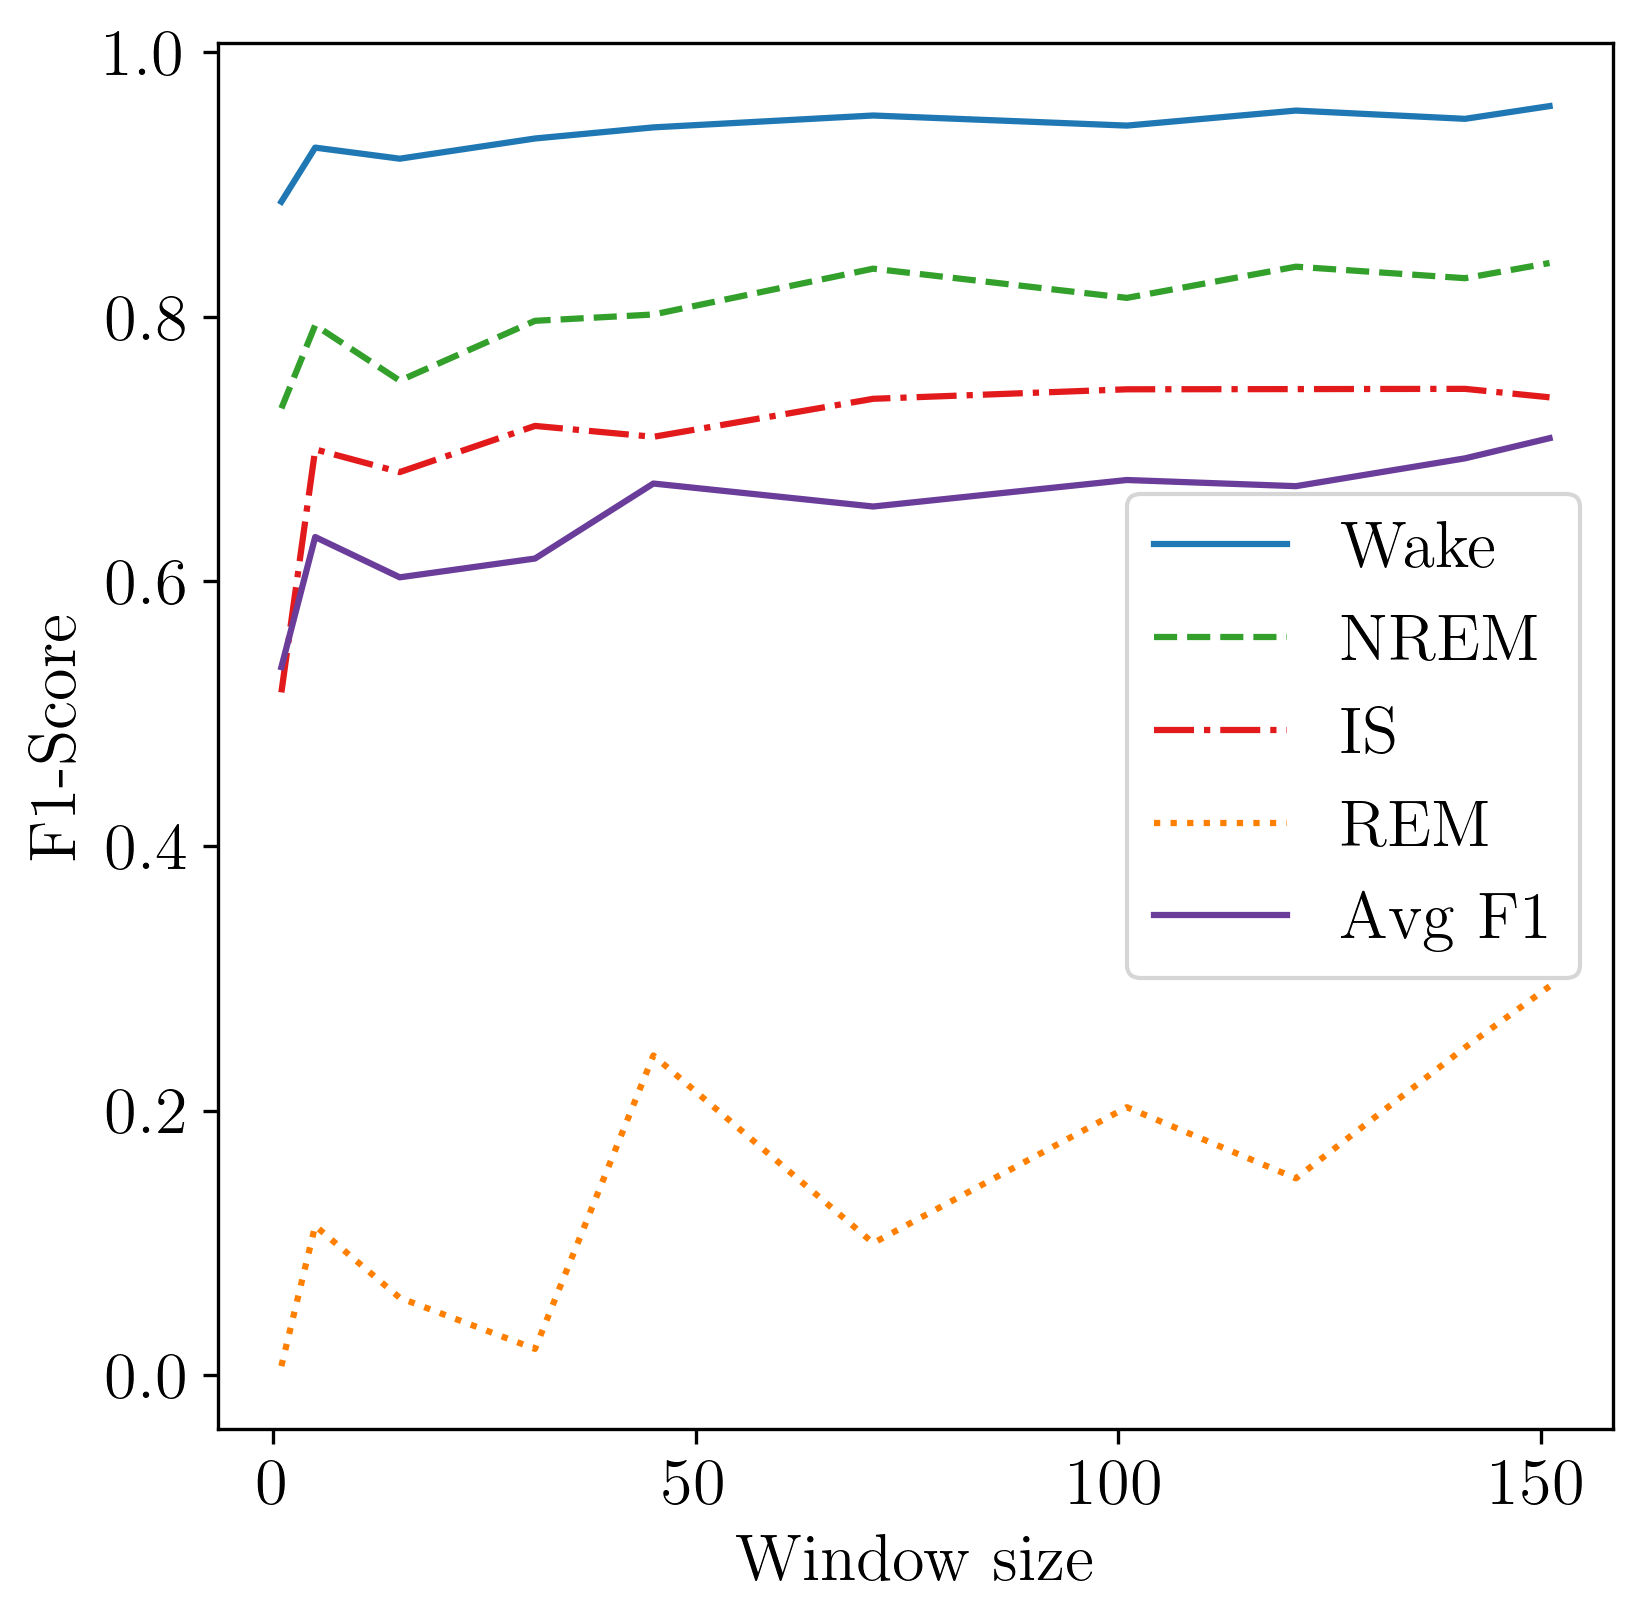
\includegraphics[width=\linewidth]{figures/1d_plot_f1_score_trial_8_mouse_b2wtm2.csv.png} 
    \caption{F1 score for all sleep stages and its averages as function of window sizes, for the specific mouse individual \texttt{B2WTM2} Network architecture: \texttt{2 hidden layers. Layer sizes: 64 and 11. Optimizer: Adam (Rho1=0.9, Rho2=0.999). Learning Rate=0.001. Cross Entropy Loss.}}
    \label{fig:window_size}
\end{figure}

In the preliminary testing, we observed greater variance in model performance when altering the window size. This trend was further confirmed during the evaluation phase, as shown in \hyperref[fig:window_size]{Figure~\ref*{fig:window_size}}. Selecting a model with a larger window size (approximately 50, corresponding to a time period of over 150 seconds) resulted in improved overall F1-score.

For all sleep stages except REM-sleep, the models stabilize as we increased the window size. However, for the REM sleep stage we can observe larger variance as we vary the window size. We attribute this to the rapid fluctuations characteristic of REM sleep, where windows size variation could include irrelevant information, potentially diluting the model's ability to identify specific patterns.

To address this, we propose a balanced approach that optimizes the tradeoff between precision and sleep stage-specific accuracy.

\subsection*{Feature Engineering and Power Ratios}
To overcome the performance plateau, we explore adding additional power ratios to the model through feature engineering. Using the preprocessing framework outlined earlier, we selectively include features with low correlation to minimize redundancy. In specific, we use \texttt{delta\_theta\_ratio}, \texttt{sigma\_beta\_ratio}, \texttt{theta\_sigma\_ratio}, \texttt{emg\_delta\_ratio}, \texttt{delta\_power}, \texttt{sigma\_power} and \texttt{emg\_power} as features.

As illustrated in Figures \hyperref[fig:ffnn_fe_cm1]{~\ref*{fig:ffnn_fe_cm1}} and \hyperref[fig:ffnn_fe_cm2]{~\ref*{fig:ffnn_fe_cm2}}, the feature-engineered model (\texttt{NNModel1O\_51}) demonstrates improvements over the original FFNN model in classifying sleep stages. Notably, the new model performs significantly better in predicting REM sleep and maintains comparable accuracy in classifying Wake and NREM stages. However, it exhibits a decline in its ability to classify IS sleep accurately. Given this tradeoff, the choice between models should be guided by the importance of accurately classifying each sleep stage for the specific application.

\subsection*{Evaluation of model \texttt{NNModel1O\_51}}
With the training stage complete, we can draw several conclusions. Among the factors considered, adjustments to the window size and feature engineering has the most significant impact on model performance. In contrast, changes to hyperparameters yield minimal improvements.

The confusion matrix in \hyperref[fig:ffnn_fe_cm1]{Figure~\ref*{fig:ffnn_fe_cm1}} along with the classification report from model \texttt{NNModel1O\_51} tested on test mouse: \texttt{trial8\_b2wtm2} outlines its overall performance and challenges across the four sleep stages: Awake, NREM, IS and REM. The overall test accuracy of 87\% reflects strong general performace. However, the report also reveals its challenges, particulary with predicting less represented sleep stages (REM, IS).

For the Wake stage, the model performs exceptionally well, with a precision of 99\% and f1-score of 94\%. The model is able to classify most Wake instances correctly. However, a small portion is misclassified as primarly REM and NREM, this is reflected by the recall of 89\%. Similarly, the model performs well on NREM, which is the class with the second most support. It achieves general high recall and F1-score, 94\% and 82\% respectively. However, the lower precision of 74\% implies some misclassifications, where other stages, especially IS and REM, are mistakenly labeled as NREM.

In contrast, predicting Intermediate Sleep proves to be a significant challenge for the model. With a precision of 77\% and a recall of 59\%, the F1-score of 67\% reflects the difficulty the model has in accurately identifying IS instances. Many true IS cases are misclassified as NREM or Wake, indicating room for improvement in capturing the unique features of this stage. 

The REM stage classification has significantly improved from the non-feature engineered models. However it still presents difficulties. The high recall of 84\% shows that the model successfully identifies most REM cases; however, the precision drops to 33\%, resulting in an F1-score of 48\%. This indicates that, while the model is sensitive to REM instances, it often misclassifies other stages as REM — particularly wake.

By feature engineering we are able to boost the REM stage classification, but it comes at a cost: a significant drop for the IS sleep stage.
\end{multicols}

\begin{figure}[H]
    \centering
    \begin{tcolorbox}[colframe=black, colback=white, sharp corners, boxrule=0.2mm, width=\textwidth]
        \begin{minipage}[t]{0.48\textwidth}
            \centering
            \includegraphics[width=\linewidth]{figures/feature_engineered_confusion 2.png}
            \caption{Model \texttt{NNModel1O\_51}\textbf{with feature engineering. }Confusion matrix for FFNN testing on feature engineered mouse data (1) for mouse model \texttt{B2WTM2, trial 8}. Hyper parameters: \texttt{2 hidden layers. Layer sizes: 64 and 11. Window size: 121. Optimizer: Adam (Rho1=0.9, Rho2=0.999). Learning Rate=0.001. Cross Entropy Loss.}}
            \label{fig:ffnn_fe_cm1}
            \vspace{0.5cm}
            {\small
            \begin{verbatim}
Classification report:
           prec.  rcl   f1  support

    Wake   0.99  0.89  0.94  30739
    NREM   0.74  0.94  0.82   8372
      IS   0.77  0.59  0.67   2834
     REM   0.33  0.84  0.48   1115

accuracy               0.87  43060
macr avg   0.71  0.81  0.73  43060
 wgt avg   0.91  0.87  0.88  43060

Accuracy of test data netw.:  87 %
Accuracy for class: Wake  is 88.6 %
Accuracy for class: NREM  is 93.6 %
Accuracy for class: IS    is 59.1 %
Accuracy for class: REM   is 84.1 %
            \end{verbatim}}
        \end{minipage}
        \hfill
        \begin{minipage}[t]{0.48\textwidth}
            \centering
            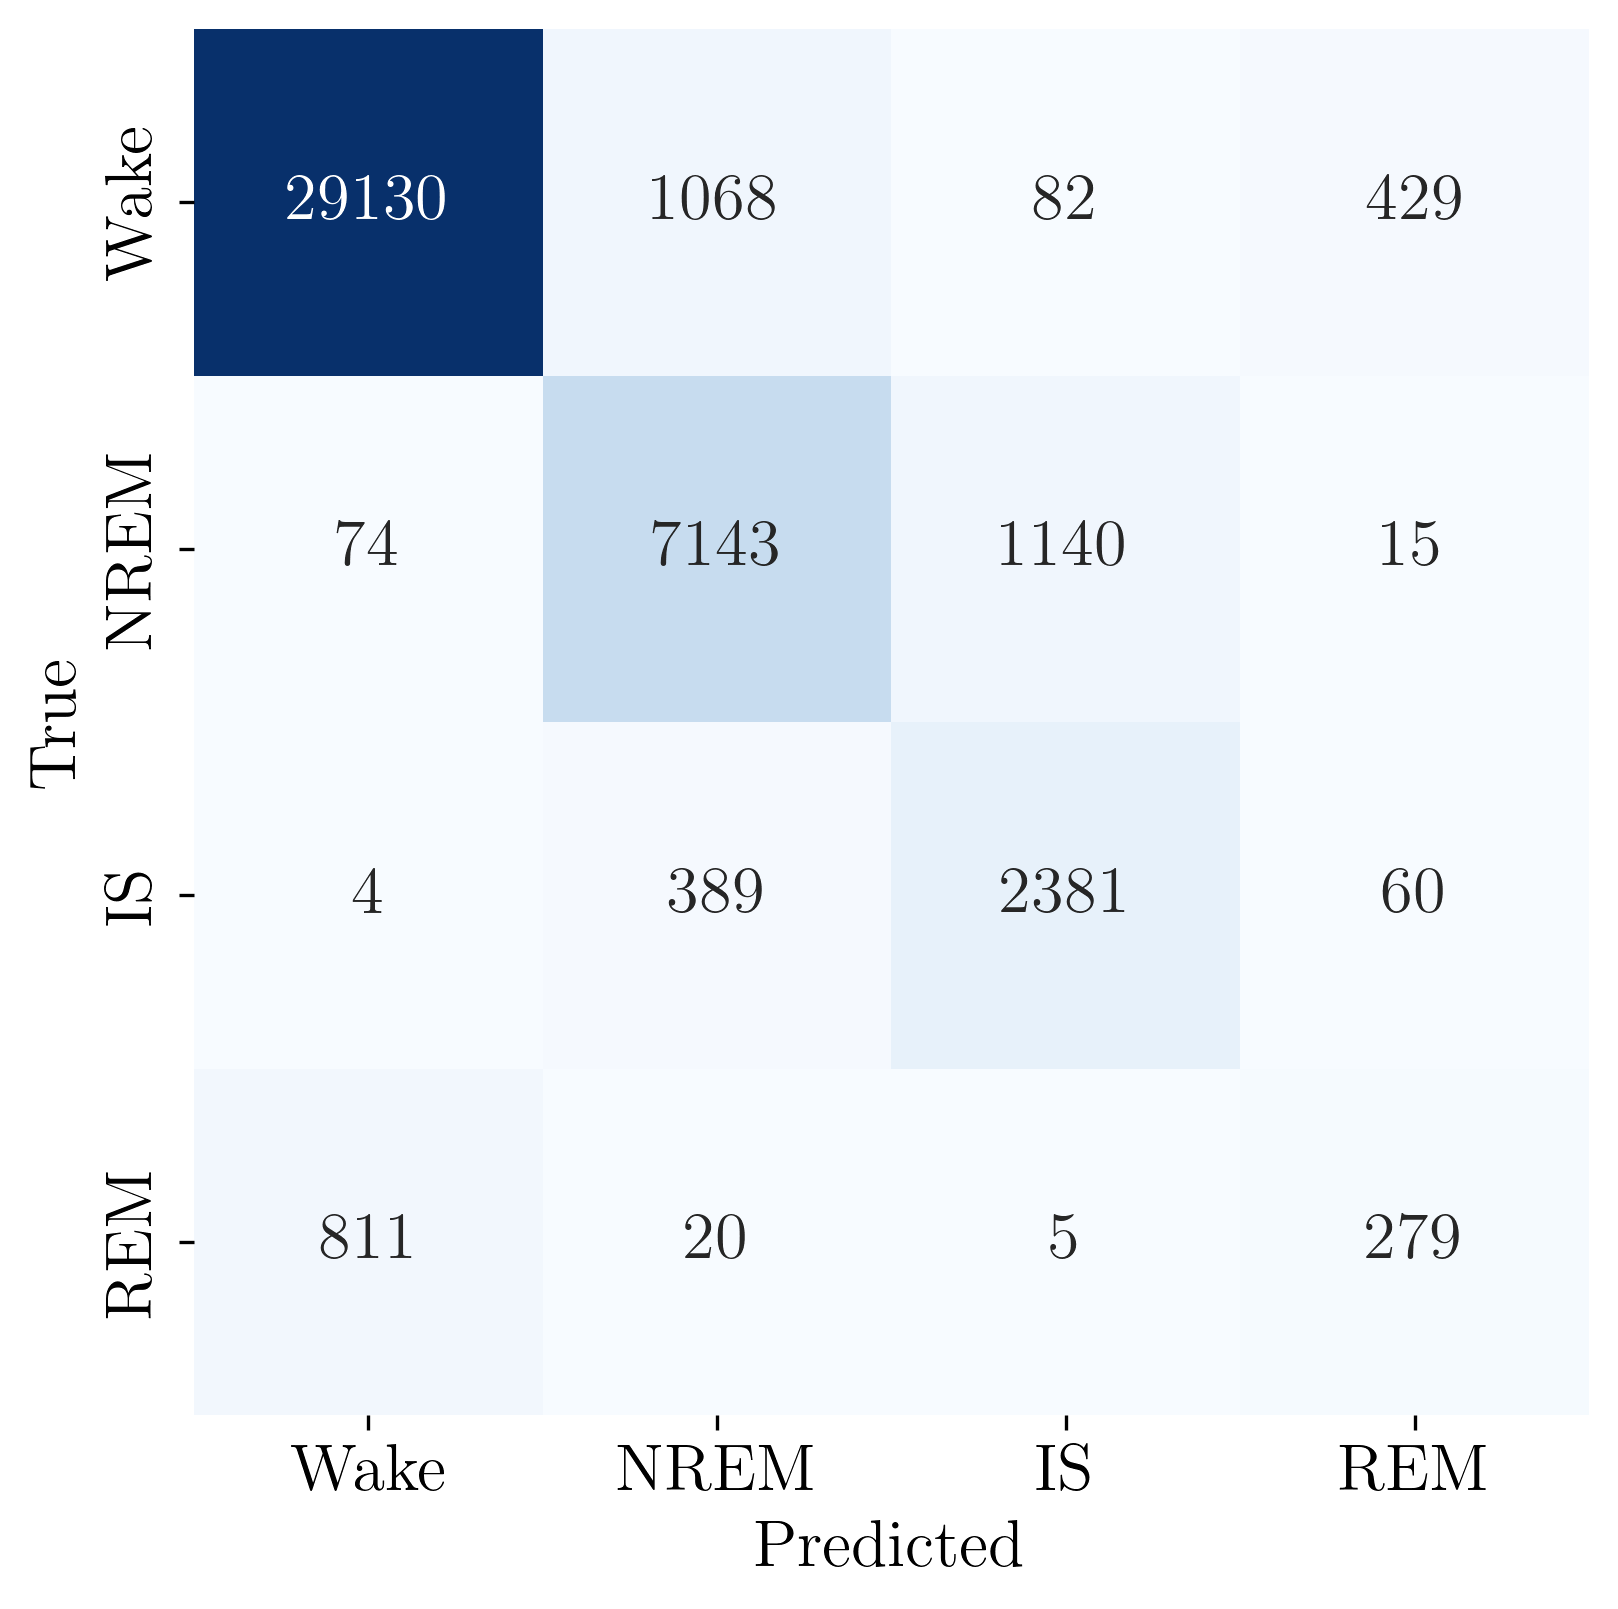
\includegraphics[width=\linewidth]{figures/confusion_matrix_model_19.png}
            \caption{\textbf{Model \texttt{NN\_Model\_1\_19} without feature engineering.} Confusion matrix for FFNN testing on ``clean'' mouse data (2) for mouse model \texttt{B2WTM2, trial 8}. Hyper parameters: \texttt{2 hidden layers. Layer sizes: 64 and 11. Window size: 121. Optimizer: Adam (Rho1=0.9, Rho2=0.999). Learning Rate=0.001. Cross Entropy Loss.}}
            \label{fig:ffnn_fe_cm2}
            \vspace{0.5cm}
            {\small
            \begin{verbatim}
Classification report:
           prec.  rcl   f1  support

    Wake   0.97  0.95  0.96  30709
    NREM   0.83  0.85  0.84   8372
      IS   0.66  0.84  0.74   2834
     REM   0.36  0.25  0.29   1115

accuracy               0.90  43030
macr avg   0.70  0.72  0.71  43030
 wgt avg   0.91  0.90  0.90  43030

Accuracy of test data netw.:   90 %
Accuracy for class: Wake  is 94.9 %
Accuracy for class: NREM  is 85.3 %
Accuracy for class: IS    is 84.0 %
Accuracy for class: REM   is 25.0 %
            \end{verbatim}}
        \end{minipage}
    \end{tcolorbox}
\end{figure}

\section*{Training the \textit{SPINDLE}-inspired CNN-model}

\begin{figure}[H]
    \centering
    \makebox[0pt][c]{\includegraphics[width=1.2\linewidth]{figures/CNN.eps}}
    \caption{1) Power data for EEGs, as well as EMG received from \textit{GliaLab}, with the corresponding labels (\texttt{sleep\_episode}). 2) Treating these frequency plots like images make the inputs in a convolutional neural network. 3) Convolution layer. 4) Pooling layer. 5) Fully connected (dense) layer. 6) Predicted classes (\texttt{REM, IS, NREM} or \texttt{Awake})}
    \label{fig:cnn}
\end{figure}

\begin{multicols}{2}
In another effort to combat the performance plateau, specifically related to the underrepresented classes REM-sleep and IS, we change the type of artifical neural network. Inspired by SPINDLE \cite{miladinovic_SPINDLE_2019} we now created a Convolutional Neural Network (CNN) using Pytorch. 

\subsection*{Creation of Images}
As a starting point, we consider the four ECoG power values and one EMG power value for a given 3-second epoch, shown in stage 1 of \hyperref[fig:cnn]{Figure~\ref*{fig:cnn}}. By stacking the ECoG power values vertically, we form a $(4\times1)$-pixel image, which serves as the foundation for one of the CNN input images.

To incorporate the EMG power value, we construct a second image by replicating the EMG power value four times in a vertical stack. This results in another  $(4\times1)$-pixel image, providing the basis for the second input to the CNN. 

To capture temporal context from surrounding sleep episodes, we extend this approach using window sizes. A window size of $n$ produces two $(4\times n)$ images. This is depicted in stage 2 of \hyperref[fig:cnn]{Figure~\ref*{fig:cnn}}.

\subsection*{Training Evaluation}
In an effort to deepen our analysis, we heuristically experiment with CNN-specific architectures. A wide range of tunable parameters are tested, including pooling configurations such as kernel sizes and the number of pooling layers. For the convolution stage, we explore variations in kernel sizes, the number of layers, and the inclusion of padding.

Our experiments reveal a consistent trend similar to that observed with the Feed Forward Neural Network (FFNN): specific structural tuning has had minimal impact on performance. Ultimately, we select model \texttt{SleepScoringCNN\_1O\_7} for further testing, as it demonstrates consistent results. 

\begin{figure}[H]
    \centering
    \includegraphics[width=\linewidth]{figures/bar_plot_kernel_size.png} 
    \caption{Accuracy given differentkernel sizes in CNNs tested on three different mouse models, \texttt{b1aqm2}, \texttt{b2wtm2}, \texttt{b1wtm2}. Hyper parameters: \texttt{2 convolutional layers. MaxPooling. Stride: 1. Padding: 2. (Layer 2 has no padding). Dense layers: 64, 16. Activation fn: ReLU. Window size: 41. Optimizer: Adam (Rho1=0.9, Rho2=0.999). Learning Rate=0.001. Cross Entropy Loss.}}
    \label{fig:kernel_sizes}
\end{figure}

\hyperref[fig:kernel_sizes]{Figure~\ref*{fig:kernel_sizes}} illustrates the network accuracies as functions of convolutional kernel sizes. It further reinforces the idea that additional tuning yields minimal impact. For a more comprehensive overview of the tested parameters, please refer to the accompanying \texttt{.csv} and \texttt{.txt files}.

\begin{figure}[H]
    \centering
    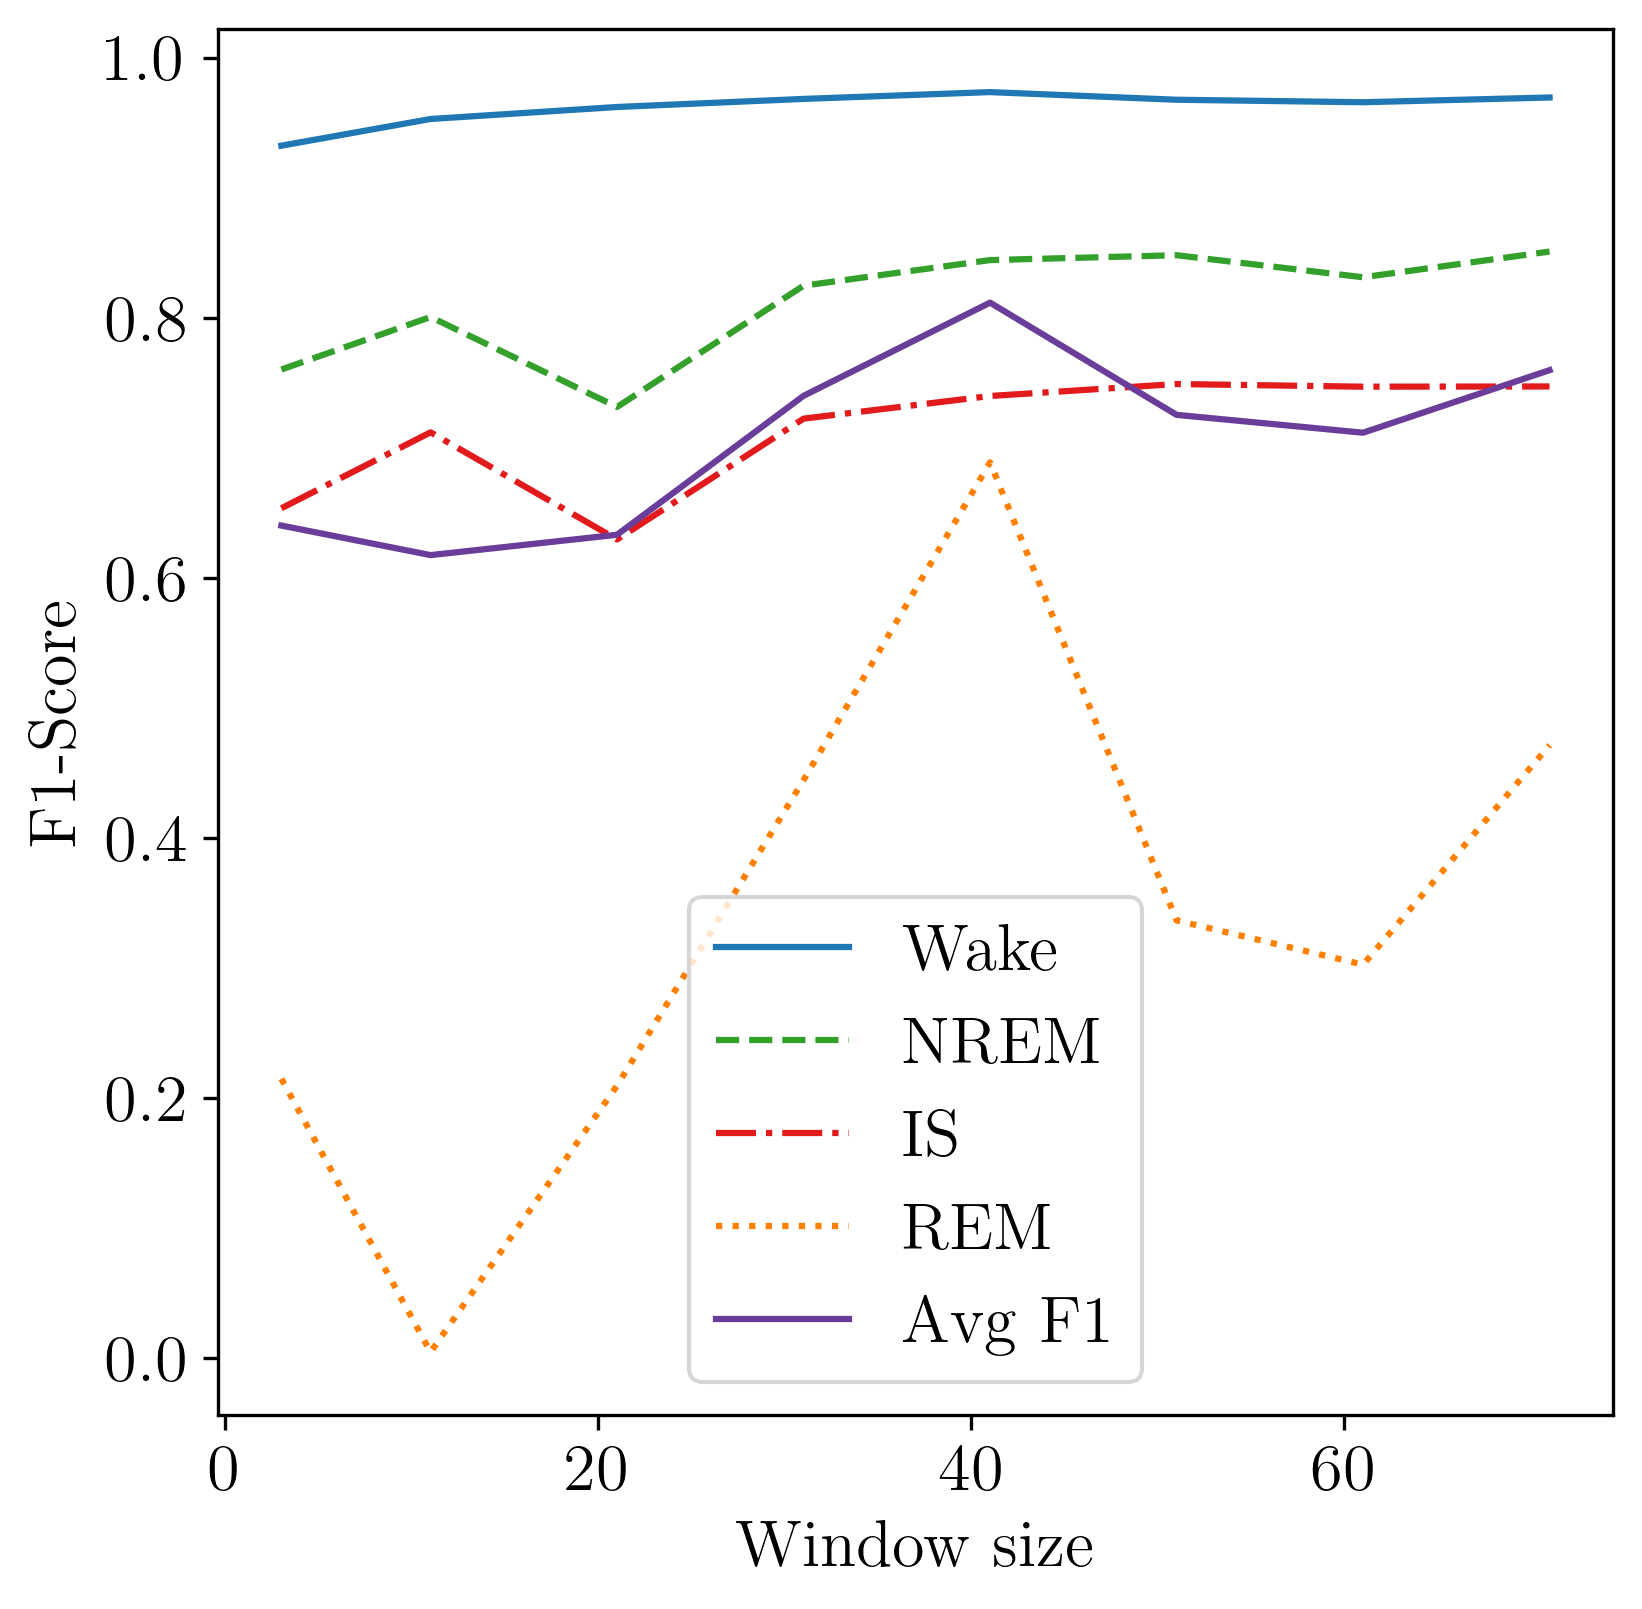
\includegraphics[width=\linewidth]{figures/1d_plot_f1_score_cnn_trial_8_mouse_b2wtm2.csv.png} 
    \caption{F1 score of varying window sizes as a function of different sleep stages in CNNs on mouse model \texttt{b2wtm2}. Hyper parameters: \texttt{2 convolutional layers. MaxPooling. Kernel size: (2x2). Stride: 1. Padding: 2. (Layer 2 has no padding). Dense layers: 64, 16. Activation fn: ReLU. Optimizer: Adam (Rho1=0.9, Rho2=0.999). Learning Rate=0.001. Cross Entropy Loss.}}
    \label{fig:window_sizes_cnn}
\end{figure}

The impact of window size is even more pronounced in the case of CNNs, as illustrated in \hyperref[fig:window_sizes_cnn]{Figure~\ref*{fig:window_sizes_cnn}}. Similar to the FFNN results, the Wake, NREM, and IS stages show only minor improvements with adjustments to window size, with a slight increase in F1-score observed for larger windows. In contrast, the REM sleep stage exhibits more significant variations. Larger window sizes initially improve the F1-score for REM sleep, but \hyperref[fig:window_sizes_cnn]{Figure~\ref*{fig:window_sizes_cnn}} reveals a clear tradeoff: when the window size exceeds 40, the F1-score for REM sleep begins to decline. We attribute this to the rapid fluctuations that characterize REM sleep. Simiarly to the behaviour in FFNN: larger window sizes may incorporate irrelevant information, diluting the model's ability to identify key patterns unique to this stage.

\subsection*{Feature Engineering}
As with the FFNN, we also explore the impact of manual feature extraction for the CNNs. Specifically, we attempt to generate a third input image incorporating specific power ratios. \hyperref[fig:cnn_fe_cm1]{Figure~\ref*{fig:cnn_fe_cm2}} shows a confusion matrix and an additional classification report for a model with \texttt{beta\_delta\_ratio}, \texttt{delta\_beta\_ratio}, \texttt{beta\_theta\_ratio} and \texttt{theta\_beta\_ratio} as the third image. Choosing the particular ratios are done with inspiration from the report \textit{Sleep-awake Classification using EEG Band-power-ratios and Complexity Measures} \cite{ganesan_sleep-awake_2020}. It suggests choosing ratios of high frequency to low frequency. In contrast to FFNNs, our manual feature engineering for CNNs do not lead to improved performance. The models trained with power ratios particularly struggle with the REM/Wake classification, a challenge that is outlined in the same mentioned report. Our testing suggests that the addition of power ratios, as a third input image, may not sufficiently address classification difficulties in these stages.

\subsection*{Concluding Training for Convolutional Neural Networks}
 Notably, we finally find the new models to outperform the FFNNs, yielding better overall validation accuracy and better performance on sleep stage-specific metrics. 

For CNNs we achieved better results with one of the fine-tuned models. In specific, we find model \texttt{CNNModel\_41W27} to provide good overall precision, also on stage-specific metrics. We will therefore evaluate this model further. 

Based on the confusion matrix in \hyperref[fig:cnn_fe_cm1]{Figure~\ref*{fig:cnn_fe_cm1}} along with the classification report for model \texttt{CNNModel\_41W27} tested on test mouse \texttt{trail8\_b2wtm2} the model demonstrates strong performance, with an accuracy of 92\%. This shows robustness in classifying sleep stages, although some class specific areas reveal room for improvement.

The model performs exceptionally well in identifying the Wake stage, achieving a precision of 98\%, recall of 96\% and an F1-score of 97\%. Its success in classifying this stage is likely aided by the large number of Wake samples in the dataset (support: 30818). Similarly, NREM classification is solid, with a precision of 87\%, recall of 82\% and F1-score of 84\%. However, the confusion matrix reveals that the model misclassifies a significant part of NREM as IS, 1322 instances in specific. 

The model's performance on IS-stage is more mixed. It achieves a high recall of 87\%, suggesting effective detection when the stage is actually present. However, the precision drops to 64\%, indicating frequent misclassifications, particulary with NREM. Furthermore, the REM-stage remains the most challenging for the model, with a precision of 65\%, recall of 74\% and F1-score of 69\%. These metrics indicate difficulty in distinguishing REM from other stages, likely due to its smaller representation in the dataset (support: 1,115) and overlapping features with other stages, especially ``Wake''.

Based on this analysis, we suggest that further improvements could be seen with increased training samples for underrepresented stages like IS and REM. Additionally, refined feature engineering methods to better capture the transitional characteristics of these stages may help reduce confusion. 

\end{multicols}
\begin{figure}[H]
    \centering
    \begin{tcolorbox}[colframe=black, colback=white, sharp corners, boxrule=0.2mm, width=\textwidth]
        \begin{minipage}[t]{0.48\textwidth}
            \centering
            \includegraphics[width=\linewidth]{figures/conf_matrix_cnn_41_window.png}
            \caption{\textbf{Without feature engineering.} Confusion matrix for \textbf{CNN} testing on mouse model \texttt{B2WTM2, trial 8} Hyper parameters: \texttt{2 convolutional layers. MaxPooling. Stride: 1. Padding: 2. (Layer 2 has no padding). Dense layers: 64, 16. Activation fn: ReLU. Window size: 41. Optimizer: Adam (Rho1=0.9, Rho2=0.999). Learning Rate=0.001. Cross Entropy Loss.}}
            \label{fig:cnn_fe_cm1}
            \vspace{0.5cm}
            {\small
        \begin{verbatim}

Classification report:
           prec.  rcl   f1  support

    Wake   0.98  0.96  0.97  30818
    NREM   0.87  0.82  0.84   8372
      IS   0.64  0.87  0.74   2834
     REM   0.65  0.74  0.69   1115

accuracy               0.92  43139
macr avg   0.79  0.85  0.81  43139
 wgt avg   0.93  0.92  0.93  43139

Accuracy of test data netw.:   92 %
Accuracy for class: Wake  is 96.3 %
Accuracy for class: NREM  is 81.8 %
Accuracy for class: IS    is 87.2 %
Accuracy for class: REM   is 73.7 %
        \end{verbatim}}
        \end{minipage}
        \hfill
        \begin{minipage}[t]{0.48\textwidth}
            \centering
            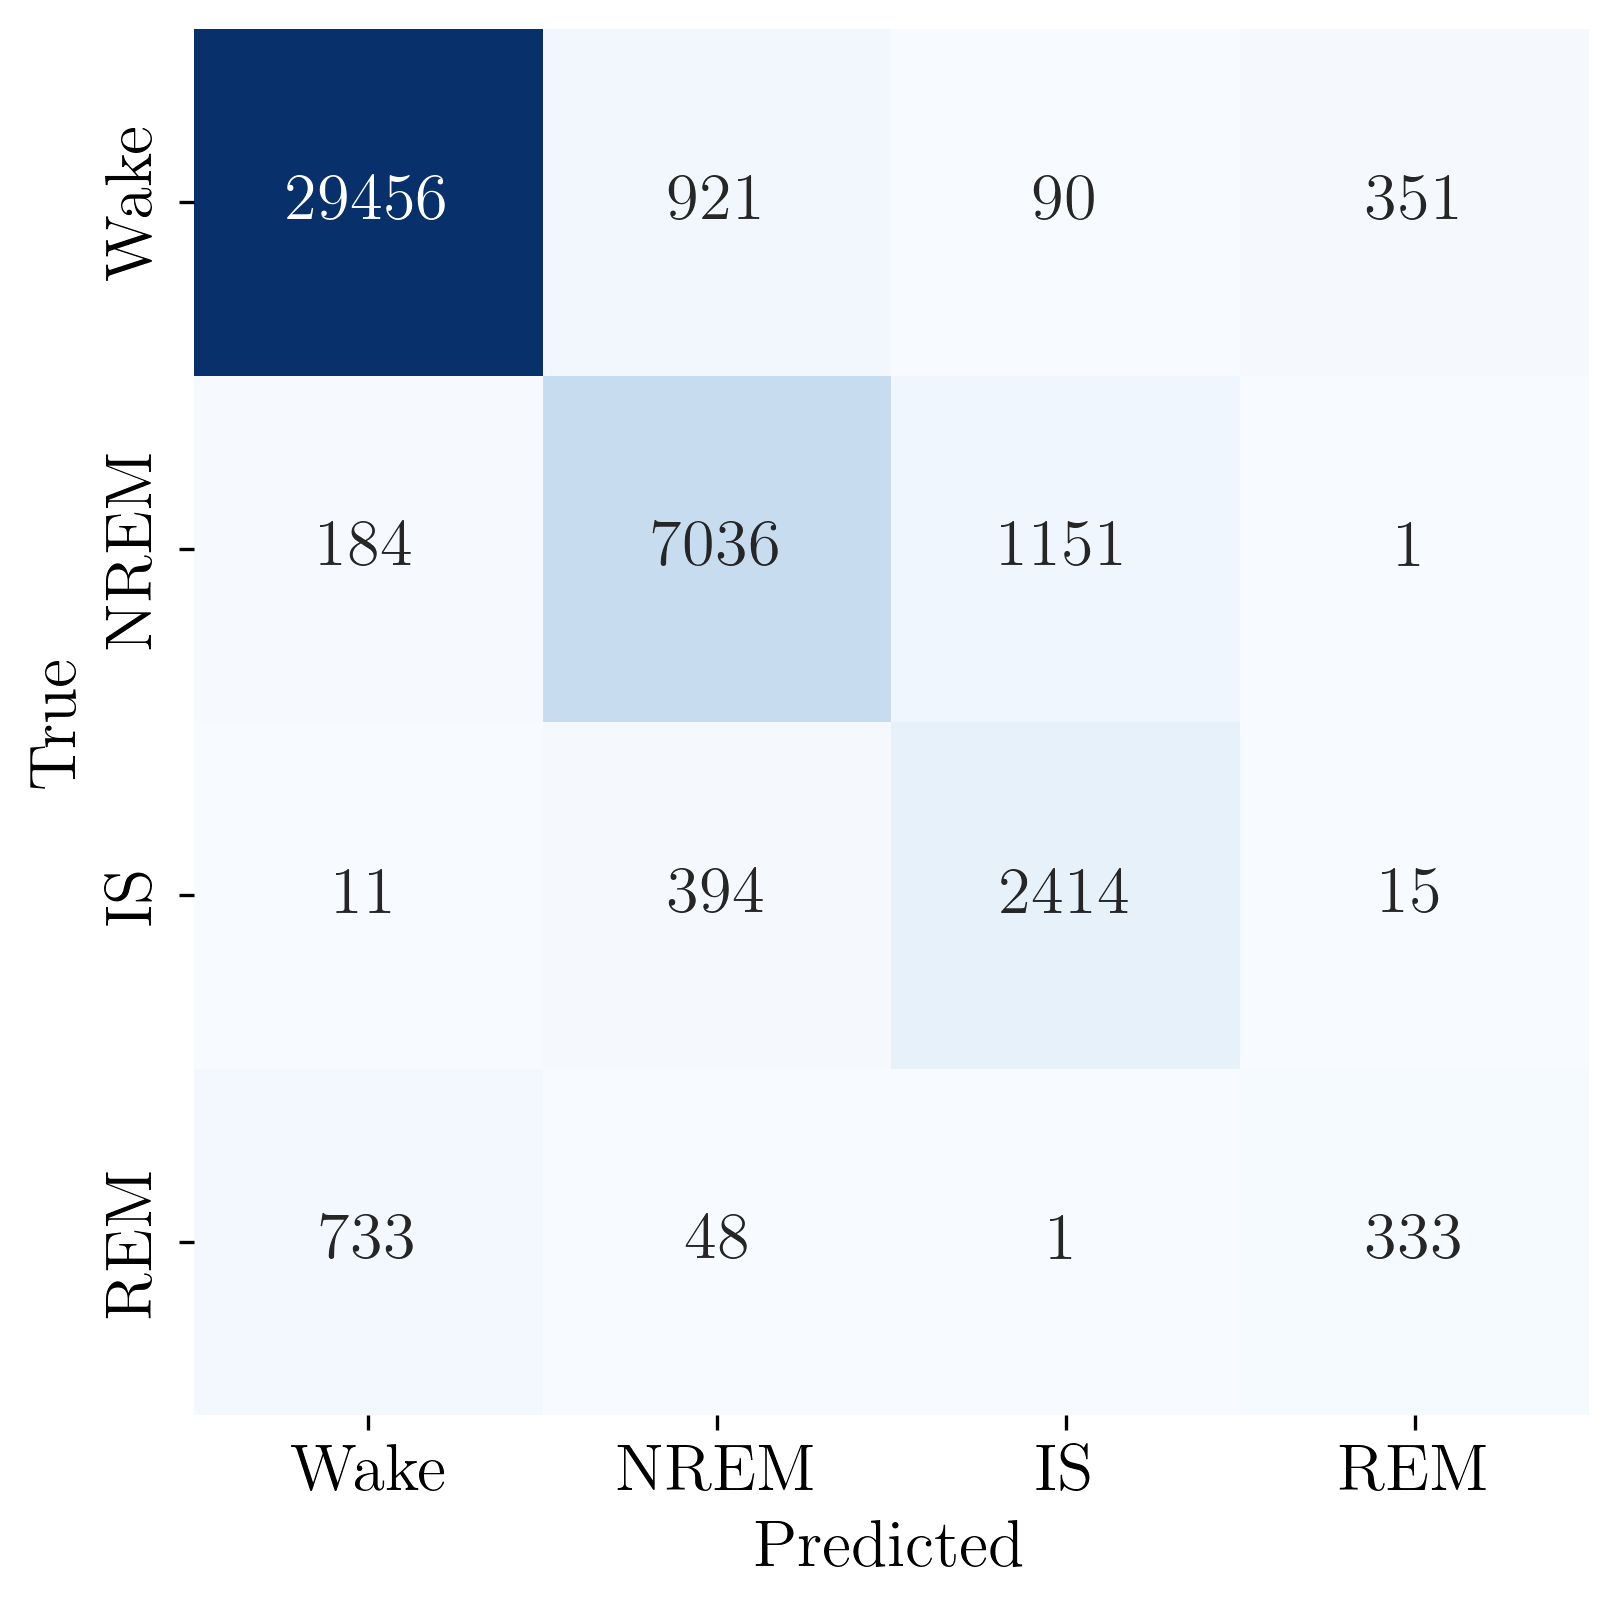
\includegraphics[width=\linewidth]{figures/conf_matrix_cnn_ratios_41_window_b2wtm2.png}
            \caption{\textbf{With feature engineering, including a third image of \texttt{power\_ratios}.} Confusion matrix for \textbf{CNN} testing on mouse model \texttt{B2WTM2, trial 8} Hyper parameters: \texttt{2 convolutional layers. MaxPooling. Stride: 1. Padding: 2. (Layer 2 has no padding). Dense layers: 64, 16. Activation fn: ReLU. Window size: 41. Optimizer: Adam (Rho1=0.9, Rho2=0.999). Learning Rate=0.001. Cross Entropy Loss.}}
            \label{fig:cnn_fe_cm2}
            \vspace{0.5cm}
            {\small
            \begin{verbatim}

Classification report:
           prec.  rcl   f1  support

    Wake   0.97  0.96  0.96  30818
    NREM   0.84  0.85  0.84   8372
      IS   0.66  0.85  0.74   2834
     REM   0.48  0.30  0.37   1115

accuracy               0.91  43139
macr avg   0.74  0.74  0.73  43139
 wgt avg   0.91  0.91  0.91  43139

Accuracy of test data netw.:   90 %
Accuracy for class: Wake  is 95.6 %
Accuracy for class: NREM  is 84.0 %
Accuracy for class: IS    is 85.2 %
Accuracy for class: REM   is 29.9 %
            \end{verbatim}}
        \end{minipage}
    \end{tcolorbox}
\end{figure}

\begin{multicols}{2}
\end{multicols}

\section*{Conclusion}

\begin{multicols}{2}
Based on our findings, we reaffirm the established notion that Feed Forward Neural Networks (FFNNs) are generally capable of learning a wide range of tasks, but often perform poorly in domain-specific scenarios. Our FFNN model achieved an accuracy of 87\% and struggled with the most challenging class, REM sleep, yielding an F1-score of only 48\%. Basic preprocessing steps such as reducing redundancies and scaling enabled us to find meaningful stage specific improvements, particularly for REM-sleep.

Motivated by this, we implemented a Convolutional Neural Network (CNN) inspired by SPINDLE. This architecture outperformed the FFNN, achieving an accuracy of 92\% and notably better REM classification for the correct window sizes (69\% for a window size of 41). However, we suspect that the limitations of our dataset — specifically its low-resolution frequency spectrum, binned into power bands — may have contributed to our comparatively lower performance relative to SPINDLE.

With more time and a deeper understanding of Digital Signal Processing, we would have extended our work by applying our own Fourier Transform to convert the raw data into the spectral domain. Additionally, we would have incorporated a Hidden Markov Model (HMM) to better capture the temporal dependencies between different sleep phases. In the preliminary work for this paper, we also began experimenting with a Recurrent Neural Network (RNN) featuring a bidirectional LSTM structure, which \textit{could} further enhance predictions by accounting for the sequence of sleep stages over time.

In the future, we would wish to explore RNNs in greater depth, alongside integrating an HMM for post-processing. Another option would be to deepen our domain knowledge in sleep scoring further. This would allow us to focus more effectively on advanced feature engineering techniques and consider approaches like Principal Component Analysis (PCA). Combined with logistic regression and potentially augmented by an HMM, such a pipeline could offer a simpler yet more efficient alternative for sleep stage classification. \cite{van_der_donckt_not_2023} 

On a final note: having reviewed numerous reports highlighting how machine learning models often struggle with a relatively simple classification task such as sleep scoring, we are prompted to consider a more philosophical question: What is it that a human sleep scorer sees in the data—and in the \textit{Alzheimer's Disease} mouse model—that a machine cannot? As we advance in this field, this question could indeed be worth remembering.
\end{multicols}

\section*{Acknowledgements}
We would like to thank \textit{GliaLab} at the Medical Department of The University of Oslo (UiO) for providing their data from trials in mouse model conducted at the Letten Center. Special thanks to Principal Investigator Rune Enger, MD, PhD for opening up the doors, and to PhD Student Vegard Broen, for providing us with the data sets, and answering all our questions along the way. Finally, a big thanks to Postdoctoral Researcher Laura Bojarskaite, PhD, who is \textit{GliaLab}'s human sleep scoring expert, and responsible for the data that we trained on.

\bibliographystyle{unsrt}
\bibliography{references}

\end{document}